%!TEX root = ../main.tex
\section{Query \& ground truth Construction}

\subsection{Synthetic Query Construction}
In this part, we will discuss how to construct synthetic queries by splitting large tables and generating the corresponding ground truth.

\noindent \textbf{Choosing Large Tables.} 
To create synthetic queries, we should always choose to use a large base table with more rows and columns. To achieve this, we first pick all the tables with both number of rows and columns larger than a threshold (\ie for Opendata, we set it as 50; for Webtable, we set it as 20) to ensure that they can be well splitted. Then, We sort these tables based on the number of their cell values and select top-20\%
as large table to be splitted.

  %In order to ensure the diversity of synthetic queries, we manually selected tables with different semantics as the base tables. \cc{Not clear}

\noindent \textbf{Splitting Large Tables.} 
%In this part, we discuss how to To generate syhthetic queries that are relatively realistic, including randomness and a certain level of difficulty. We mainly use two methods to generate synthetic queries for join and union case, which involve horizontal and vertical table splitting. 
At a high level, we synthesize queries for union and join by  horizontally and vertically splitting the chosen large tables.

\begin{figure}[h]
	\centering
	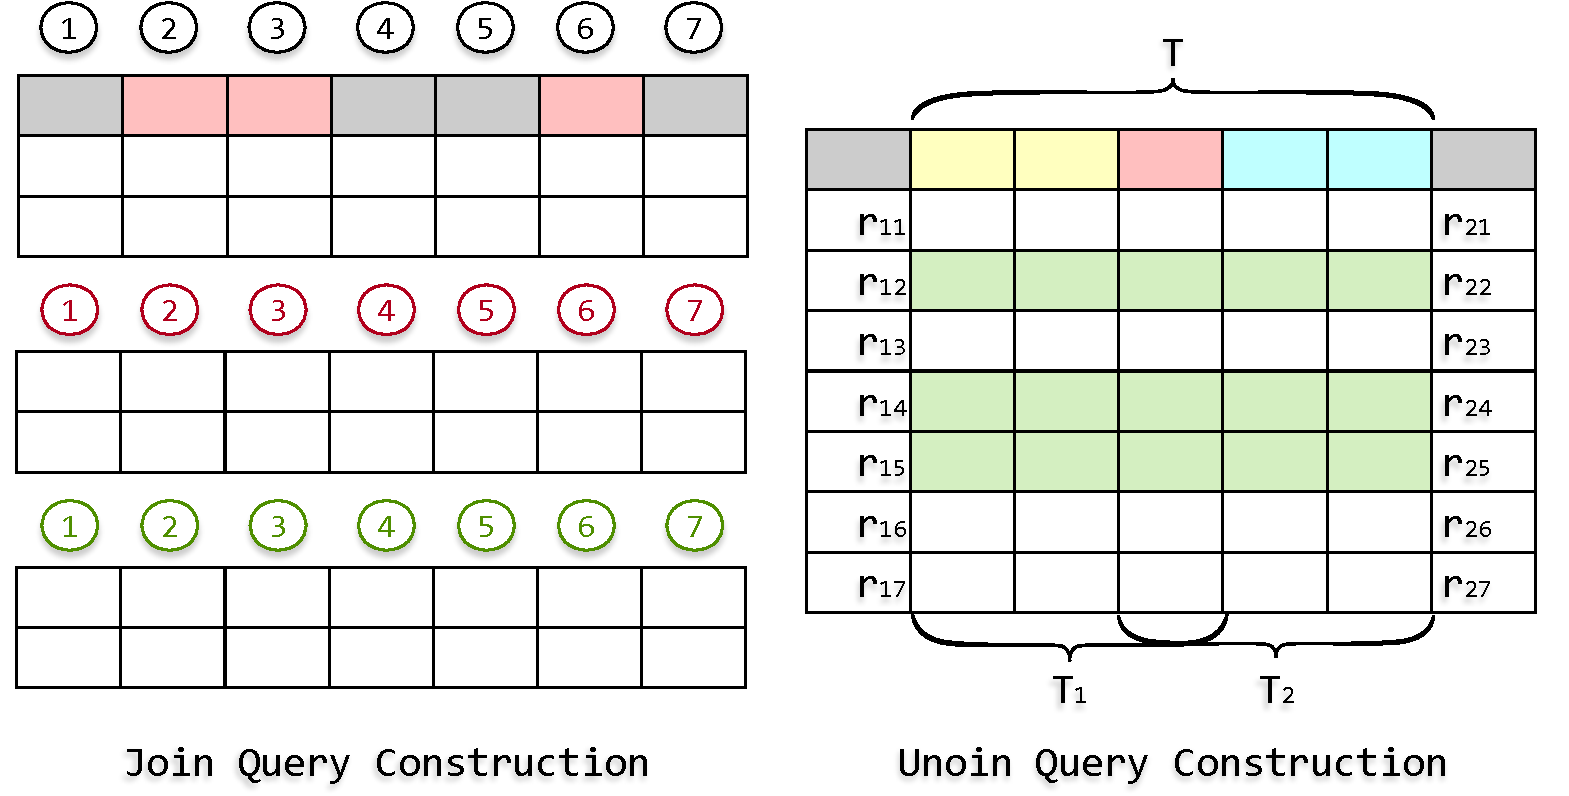
\includegraphics[width=1\linewidth]{fig/fake_query.pdf}
	\caption{Examples of Synthetic Query Construction.}
	\label{fig:query_construction}
\end{figure}


\noindent \underline{\textit{Union Query Construction.}}
 For a pair of unionable tables, it is essential for them to share columns from the same domain. 
  Consequently, to synthesize queries from a large table, we can randomly select multiple columns to be unioned and then split  horizontally. Specifically, let us illustrate this in detail with an an example (Figure~\ref{fig:query_construction}(a)). 
  %
  First, the three red columns are randomly selected, and then the large table is randomly splitted into three parts. In the Figure, we use   \raisebox{.3pt}{\textcircled{\hspace{-0.08cm} \raisebox{-.5pt}{1}}},
   \textcolor{red}{\raisebox{.3pt}{\textcircled{\hspace{-0.08cm} \raisebox{-.5pt}{2}}}},
  \textcolor{green}{\raisebox{.3pt}{\textcircled{\hspace{-0.08cm} \raisebox{-.5pt}{3}}}} to represent the first, second and third columns of the three parts respectively.
  %
  Second, in each part, we randomly select other  columns as supplementary columns for each part as a synthetic query. For example, in the first part we randomly select \raisebox{.3pt}{\textcircled{\hspace{-0.08cm} \raisebox{-.5pt}{1}}}\raisebox{.3pt}{\textcircled{\hspace{-0.08cm} \raisebox{-.5pt}{4}}}, combining with \raisebox{.3pt}{\textcircled{\hspace{-0.08cm} \raisebox{-.5pt}{2}}}\raisebox{.3pt}{\textcircled{\hspace{-0.08cm} \raisebox{-.5pt}{3}}}\raisebox{.3pt}{\textcircled{\hspace{-0.08cm} \raisebox{-.5pt}{6}}} 
  the table [\raisebox{.3pt}{\textcircled{\hspace{-0.08cm} \raisebox{-.5pt}{1}}}\raisebox{.3pt}{\textcircled{\hspace{-0.08cm} \raisebox{-.5pt}{2}}}\raisebox{.3pt}{\textcircled{\hspace{-0.08cm} \raisebox{-.5pt}{3}}}\raisebox{.3pt}{\textcircled{\hspace{-0.08cm} \raisebox{-.5pt}{4}}}\raisebox{.3pt}{\textcircled{\hspace{-0.08cm} \raisebox{-.5pt}{6}}}] can be a synthesized query. 
  %
  Similarly, we select  \textcolor{red}{\raisebox{.3pt}{\textcircled{\hspace{-0.08cm} \raisebox{-.5pt}{1}}}}\textcolor{red}{\raisebox{.3pt}{\textcircled{\hspace{-0.08cm} \raisebox{-.5pt}{5}}}} from the second part, 
  \textcolor{green}{\raisebox{.3pt}{\textcircled{\hspace{-0.08cm} \raisebox{-.5pt}{7}}}} from the third part, and then
  [\raisebox{.3pt}{\textcircled{\hspace{-0.08cm} \raisebox{-.5pt}{1}}}\raisebox{.3pt}{\textcircled{\hspace{-0.08cm} \raisebox{-.5pt}{2}}}\raisebox{.3pt}{\textcircled{\hspace{-0.08cm} \raisebox{-.5pt}{3}}}\raisebox{.3pt}{\textcircled{\hspace{-0.08cm} \raisebox{-.5pt}{4}}}\raisebox{.3pt}{\textcircled{\hspace{-0.08cm} \raisebox{-.5pt}{6}}}],
  [\textcolor{red}{\raisebox{.3pt}{\textcircled{\hspace{-0.08cm} \raisebox{-.5pt}{1}}}}\textcolor{red}{\raisebox{.3pt}{\textcircled{\hspace{-0.08cm} \raisebox{-.5pt}{2}}}}\textcolor{red}{\raisebox{.3pt}{\textcircled{\hspace{-0.08cm} \raisebox{-.5pt}{3}}}}\textcolor{red}{\raisebox{.3pt}{\textcircled{\hspace{-0.08cm} \raisebox{-.5pt}{5}}}}\textcolor{red}{\raisebox{.3pt}{\textcircled{\hspace{-0.08cm} \raisebox{-.5pt}{6}}}}]
   and
  [\textcolor{green}{\raisebox{.3pt}{\textcircled{\hspace{-0.08cm} \raisebox{-.5pt}{2}}}}\textcolor{green}{\raisebox{.3pt}{\textcircled{\hspace{-0.08cm} \raisebox{-.5pt}{3}}}}\textcolor{green}{\raisebox{.3pt}{\textcircled{\hspace{-0.08cm} \raisebox{-.5pt}{6}}}}\textcolor{green}{\raisebox{.3pt}{\textcircled{\hspace{-0.08cm} \raisebox{-.5pt}{7}}}}] are three tables that can be unioned with each other. 
  Generally speaking, we can randomly identify columns to be unioned in  each large table  for multiple times and the number of such columns, splits, and supplementary columns are also randomly chosen to ensure diverse queries. 
  
  \cc{add some difficulties.}
  
  
  
 %We first select several columns randomly from base table as column overlap (i.e. column \raisebox{.3pt}{\textcircled{\hspace{-0.08cm} \raisebox{-.5pt}{2}}}, column \raisebox{.3pt}{\textcircled{\hspace{-0.08cm} \raisebox{-.5pt}{3}}} and column \raisebox{.3pt}{\textcircled{\hspace{-0.08cm} \raisebox{-.5pt}{6}}}). Next, we proceed by horizontally splitting the table into multiple parts. 
 %
% Following this, we select the remaining non-duplicate columns as supplementary columns for each part, creating the synthetic queries for the union case. 
 %
 % In the example of the figure, we divide the large table into three parts, for the first part, we choose column \raisebox{.3pt}{\textcircled{\hspace{-0.08cm} \raisebox{-.5pt}{1}}} and column \raisebox{.3pt}{\textcircled{\hspace{-0.08cm} \raisebox{-.5pt}{6}}},  add to those overlap columns. In the same way, for the second part, we select column \raisebox{.3pt}{\textcircled{\hspace{-0.08cm} \raisebox{-.5pt}{4}}} and column \raisebox{.3pt}{\textcircled{\hspace{-0.08cm} \raisebox{-.5pt}{5}}}, for the last part, we select column \raisebox{.3pt}{\textcircled{\hspace{-0.08cm} \raisebox{-.5pt}{5}}} and column \raisebox{.3pt}{\textcircled{\hspace{-0.08cm} \raisebox{-.5pt}{7}}}. The tables formed by each part can be unioned with each other.

\noindent \underline{\textit{Join Query Construction.}}  For a pair of joinable tables, they should respectively have one column to be joined and basically, the two columns should  exhibit a substantial \cc{row} overlap. To achieve this, as shown in Figure~\ref{fig:query_construction}(b), we first randomly select a  column (highlighted as red) as the joinable column. 
%%
Subsequently, we randomly select of yellow columns to form table $T_1$, and another set of blue columns  is randomly chosen to form  $T_2$. At a high level, the pair of joinable tables are respectively sampled from $T_1$ and $T_2$ 
(we use $T$ to denote the combination table of $T_1$ and $T_2$, and $r_{1i}$ denotes the $i$-th row in $T_1$ ).
%
To create the overlaps, we randomly select some row from  $T$ as overlapping rows, marked as green. Next, we  randomly choose a set of rows  from   $T_1$ and  $T_2$, and append them to the overlapping rows.
If $r_{11}, r_{13}$ ($r_{26}, r_{27}$) are selected from $T_1$ ($T_2$), we create two queries [$r_{11}, r_{12}, r_{13}, r_{14}, r_{15}$] and  [$r_{22}, r_{24}, r_{25}, r_{26}, r_{27}$] that can be joined with each other.

 % For $T_1$ and $T_2$, we represent their rows as $r_{1x}$ and $r_{2x}$ respectively, where $x$ represents the row number. Additionally, we randomly select several columns from  $T$ to create row overlap. Next, we choose a set of rows randomly from both  $T_1$ and  $T_2$, and append them to the overlapping rows. For example, selecting $r_{11}$ from $T_1$ and choose $r_{26}$ as well as $r_{27}$ from $T_2$, allows these two tables to be joined.
  
  
\cc{add some difficulties.}

\noindent \textbf{Ground Truth Generation.} 
The  ground truth of synthesized queries can be derived from  three perspectives.

%During the process of constructing synthetic queries, ground truth are also generated accordingly.

\noindent \underline{\textit{Union Ground Truth Generation.}}  
First, as mentioned above, given multiple red columns, the splitted tables are unionable with each other.
%
%we randomly partitioned the large table into several smaller tables, all sharing the same columns. Consequently, these tables are pair-wise unionable, forming the basis for our ground truth.
%
Second, since we can randomly identify red columns multiple times within each large table. If in different times, duplicated columns are selected, then  splitted small tables among these different times can also be unioned.
%
%Second, since we might randomly identify columns multiple times within each large table, if there is a duplicate between the first and second set of selected identical columns, the resulting small tables from the second split and the ones from the first split can also be unioned. Consequently, additional corresponding ground truth can be generated.
%To illustrate, consider Figure~\ref{fig:query_construction}(a). In the first round, we selecte columns \raisebox{.3pt}{\textcircled{\hspace{-0.08cm} \raisebox{-.5pt}{2}}}, \raisebox{.3pt}{\textcircled{\hspace{-0.08cm} \raisebox{-.5pt}{3}}}, \raisebox{.3pt}{\textcircled{\hspace{-0.08cm} \raisebox{-.5pt}{6}}} as the column overlap, and columns \raisebox{.3pt}{\textcircled{\hspace{-0.08cm} \raisebox{-.5pt}{2}}}, \raisebox{.3pt}{\textcircled{\hspace{-0.08cm} \raisebox{-.5pt}{4}}}, \raisebox{.3pt}{\textcircled{\hspace{-0.08cm} \raisebox{-.5pt}{6}}} in the second round. Consequently, columns \raisebox{.3pt}{\textcircled{\hspace{-0.08cm} \raisebox{-.5pt}{2}}} and \raisebox{.3pt}{\textcircled{\hspace{-0.08cm} \raisebox{-.5pt}{6}}} can be unioned between the small tables split in the second round and those split in the first round. Therefore, we can label them as ground truth.
%



% In the first category, as previously mentioned, we randomly partitioned the large table into several smaller tables, all sharing the same columns. Consequently, these tables are pair-wise unionable, forming the basis for our ground truth. For the second category, since we might randomly identify columns multiple times within each large table, if there is a duplicate between the first and second set of selected identical columns, the resulting small tables from the second split and the ones from the first split can also be unioned. Consequently, additional corresponding ground truth can be generated.
% To illustrate, consider Figure~\ref{fig:query_construction}(a). In the first round, we selecte columns \raisebox{.3pt}{\textcircled{\hspace{-0.08cm} \raisebox{-.5pt}{2}}}, \raisebox{.3pt}{\textcircled{\hspace{-0.08cm} \raisebox{-.5pt}{3}}}, \raisebox{.3pt}{\textcircled{\hspace{-0.08cm} \raisebox{-.5pt}{6}}} as the column overlap, and columns \raisebox{.3pt}{\textcircled{\hspace{-0.08cm} \raisebox{-.5pt}{2}}}, \raisebox{.3pt}{\textcircled{\hspace{-0.08cm} \raisebox{-.5pt}{4}}}, \raisebox{.3pt}{\textcircled{\hspace{-0.08cm} \raisebox{-.5pt}{6}}} in the second round. Consequently, columns \raisebox{.3pt}{\textcircled{\hspace{-0.08cm} \raisebox{-.5pt}{2}}} and \raisebox{.3pt}{\textcircled{\hspace{-0.08cm} \raisebox{-.5pt}{6}}} can be unioned between the small tables split in the second round and those split in the first round. Therefore, we can label them as ground truth. 

The third category follows a process similar to generating ground truth for real queries. In the synthetic queries we construct, there might be several tables in the data lake that can be unioned with them. In this category, we are also required to retrieve a selection of candidate tables that show a relatively high relevance to the query table. Subsequently, human experts manually inspect these candidates to check their relevance.

\noindent \underline{\textit{Join Ground Truth Generation.}} 
Similarly, when constructing the synthetic quries for join case, we initially select a column as the joinable column, the choosen column and partition tables correspond to the query table and ground truth of the join case respectively. Also, when selecting the same join column, we might also choose different rows as overlap from table $T$ multiple times. If there are duplicates between the first and second set of selected rows, the initially split small table and the subsequently split small table can also be joined and marked as ground truth. Similiarly, for the synthetic query tables for join case, we continue the process by searching for tables within the data lake that exhibit high similarity. Subsequently, we manually evaluate whether these tables can be joined with the constructed query table. If they are joinable, they are also incorporated into the ground truth.


% For the second category, since we might randomly identify columns multiple times within each large table, if there is a duplicate between the first and second set of selected identical columns, the resulting small tables from the second split and the ones from the first split can also be unioned. Consequently, additional corresponding ground truth can be generated. 
 

%+ How to choose large tables.

%+ How to split.

%+ How to generate the ground truth.
\subsection{Basic Search for Candidate Generation}
In this part, for each synthetic or real query, we design a basic search algorithm to retrieve  candidate joinable/unionable tables from the data lake. 

\noindent \underline{\textit{Union Candidate Generation.}}  
To retrieve the unionable tables from the data lake, it not only requires considering $(\romannumeral1 ).$  the semantics of the corresponding columns in two tables (i.e. only considering the semantics between individual column pairs), but also $(\romannumeral2 ).$ the semantics between two tables (i.e. the relationships and semantics between different columns in the same table),  Therefore, we used multiple methods that consider these two semantics separately to obtain results on the query table. Specifically, we use \starmie,\santos and SATO. After that, we take the union of these results as the candidate tables and label them by experts.

\noindent \underline{\textit{Join Candidate Generation.}}  
In the case of joining tables, several considerations are essential:$(\romannumeral1).$ the semantics of corresponding columns in both tables. $(\romannumeral2).$ analyzing the relationship between the two tables, $(\romannumeral3).$ ensuring there is an overlap in cell values between the corresponding columns. Consequently, We used method that considers both $\romannumeral1$ and $\romannumeral2$, namely \deepjoin, and method that considers $\romannumeral3$, namely \josie, to obtain candidate tables respectively.

\noindent  \underline{\textit{Number of Candidate Tables.}}  The number of candidate tables we obtained was determined by experts. We first set an accuracy threshold (i.e. 70\%), and then manually judged that when the number of candidate tables reached a certain number, their corresponding accuracy was lower than the threshold we set. At this point, the number of selected tables is the final number of our candidate tables.
%+ How to guarantee high recall

%+ Details

\subsection{Human Labeling}
In this part, we ask the human experts to label the candidates for each query. In order to improve the efficiency of experts data labeling, we built a webpage for labeling the ground truth of both join and union case.

%+ Example shown to the experts.

\noindent \textbf{Labeling Interface.} 
The labeling interface we built is shown in the Figure ~\ref{fig:interface}, We demonstrate the interface designed for the join case and the interface for the union case follows a similar structure. The interface is primarily divided into three sections , each serving distinct functions. Next, we will elaborate on the functionality of each section.

\noindent \underline{\textit{Query Table Information.}}  
As shown in Figure ~\ref{fig:interface}-\raisebox{.3pt}{\textcircled{\hspace{-0.08cm} \raisebox{-.5pt}{1}}}, this section 
displays the main information of a specific query table, including the metadata associated with it and the progress of the labeling process. The table information  includes its corresponding metadata and the table itself. We can see that for the query table $BuildInfo.csv$, its column names varying from $CSDUID$ to $OriginalValue$. Furthermore, the column $Building Type$ predominantly contains four distinct cell values, such as $Commercial$ and $Industrial$. These meta information are displayed above the query table, serving as supplementary information to assist users in  evaluating whether two tables can be successfully joined or unioned. Beneath the query table, there is a progress bar featuring a green line indicating that 30\% of the query tables have been labeled, and the blue line indicating that 30\% of the query tables are currently undergoing the labeling process.

\noindent \underline{\textit{Set of Candidate Tables.}} This section presents comprehensive details of all candidate tables corresponding to the query table. As shown in Figure ~\ref{fig:interface}-\raisebox{.3pt}{\textcircled{\hspace{-0.08cm} \raisebox{-.5pt}{2}}}, there are three candidate tables, denoted as $Build.csv$, $BuildIntro.csv$ and $SchoolBuild.csv$. Each candidate table is accompanied by a labeling area where users can select two columns from both the query and candidate tables that can be joined, such as $BuildInfo.CSD$ and $Build.CSD$. Given the semantic similarity and overlap between these two columns, they are categorized as joinable types. Upon clicking the "add" button, the interface records and stores this labeled data in the backend database.

\noindent \underline{\textit{Set of Result.}} In this section of the interface, all the annotated data corresponding to the candidate tables is displayed, as illustrated in Figure ~\ref{fig:interface}-\raisebox{.3pt}{\textcircled{\hspace{-0.08cm} \raisebox{-.5pt}{3}}}. For instance, in the case of query table $BuildInfo.csv$ and candidate table $Build.csv$, it is evident that the $Period$ column in the query table only contains year information, whereas the  $Period$ column in the candidate table includes both year and month details, resulting in a lack of overlap between these two columns. Therefore, the labeled information indicates that these two columns cannot be joined (where "no" indicates they cannot be joined, and "yes" indicates they can be joined).
Furthermore, the interface provides a "delete" button to rectify any incorrectly labeled data. Additionally, users can review incomplete data through the page flipping function located below the candidate table, ensuring a thorough evaluation process.




\begin{figure*}[h]
	\centering
	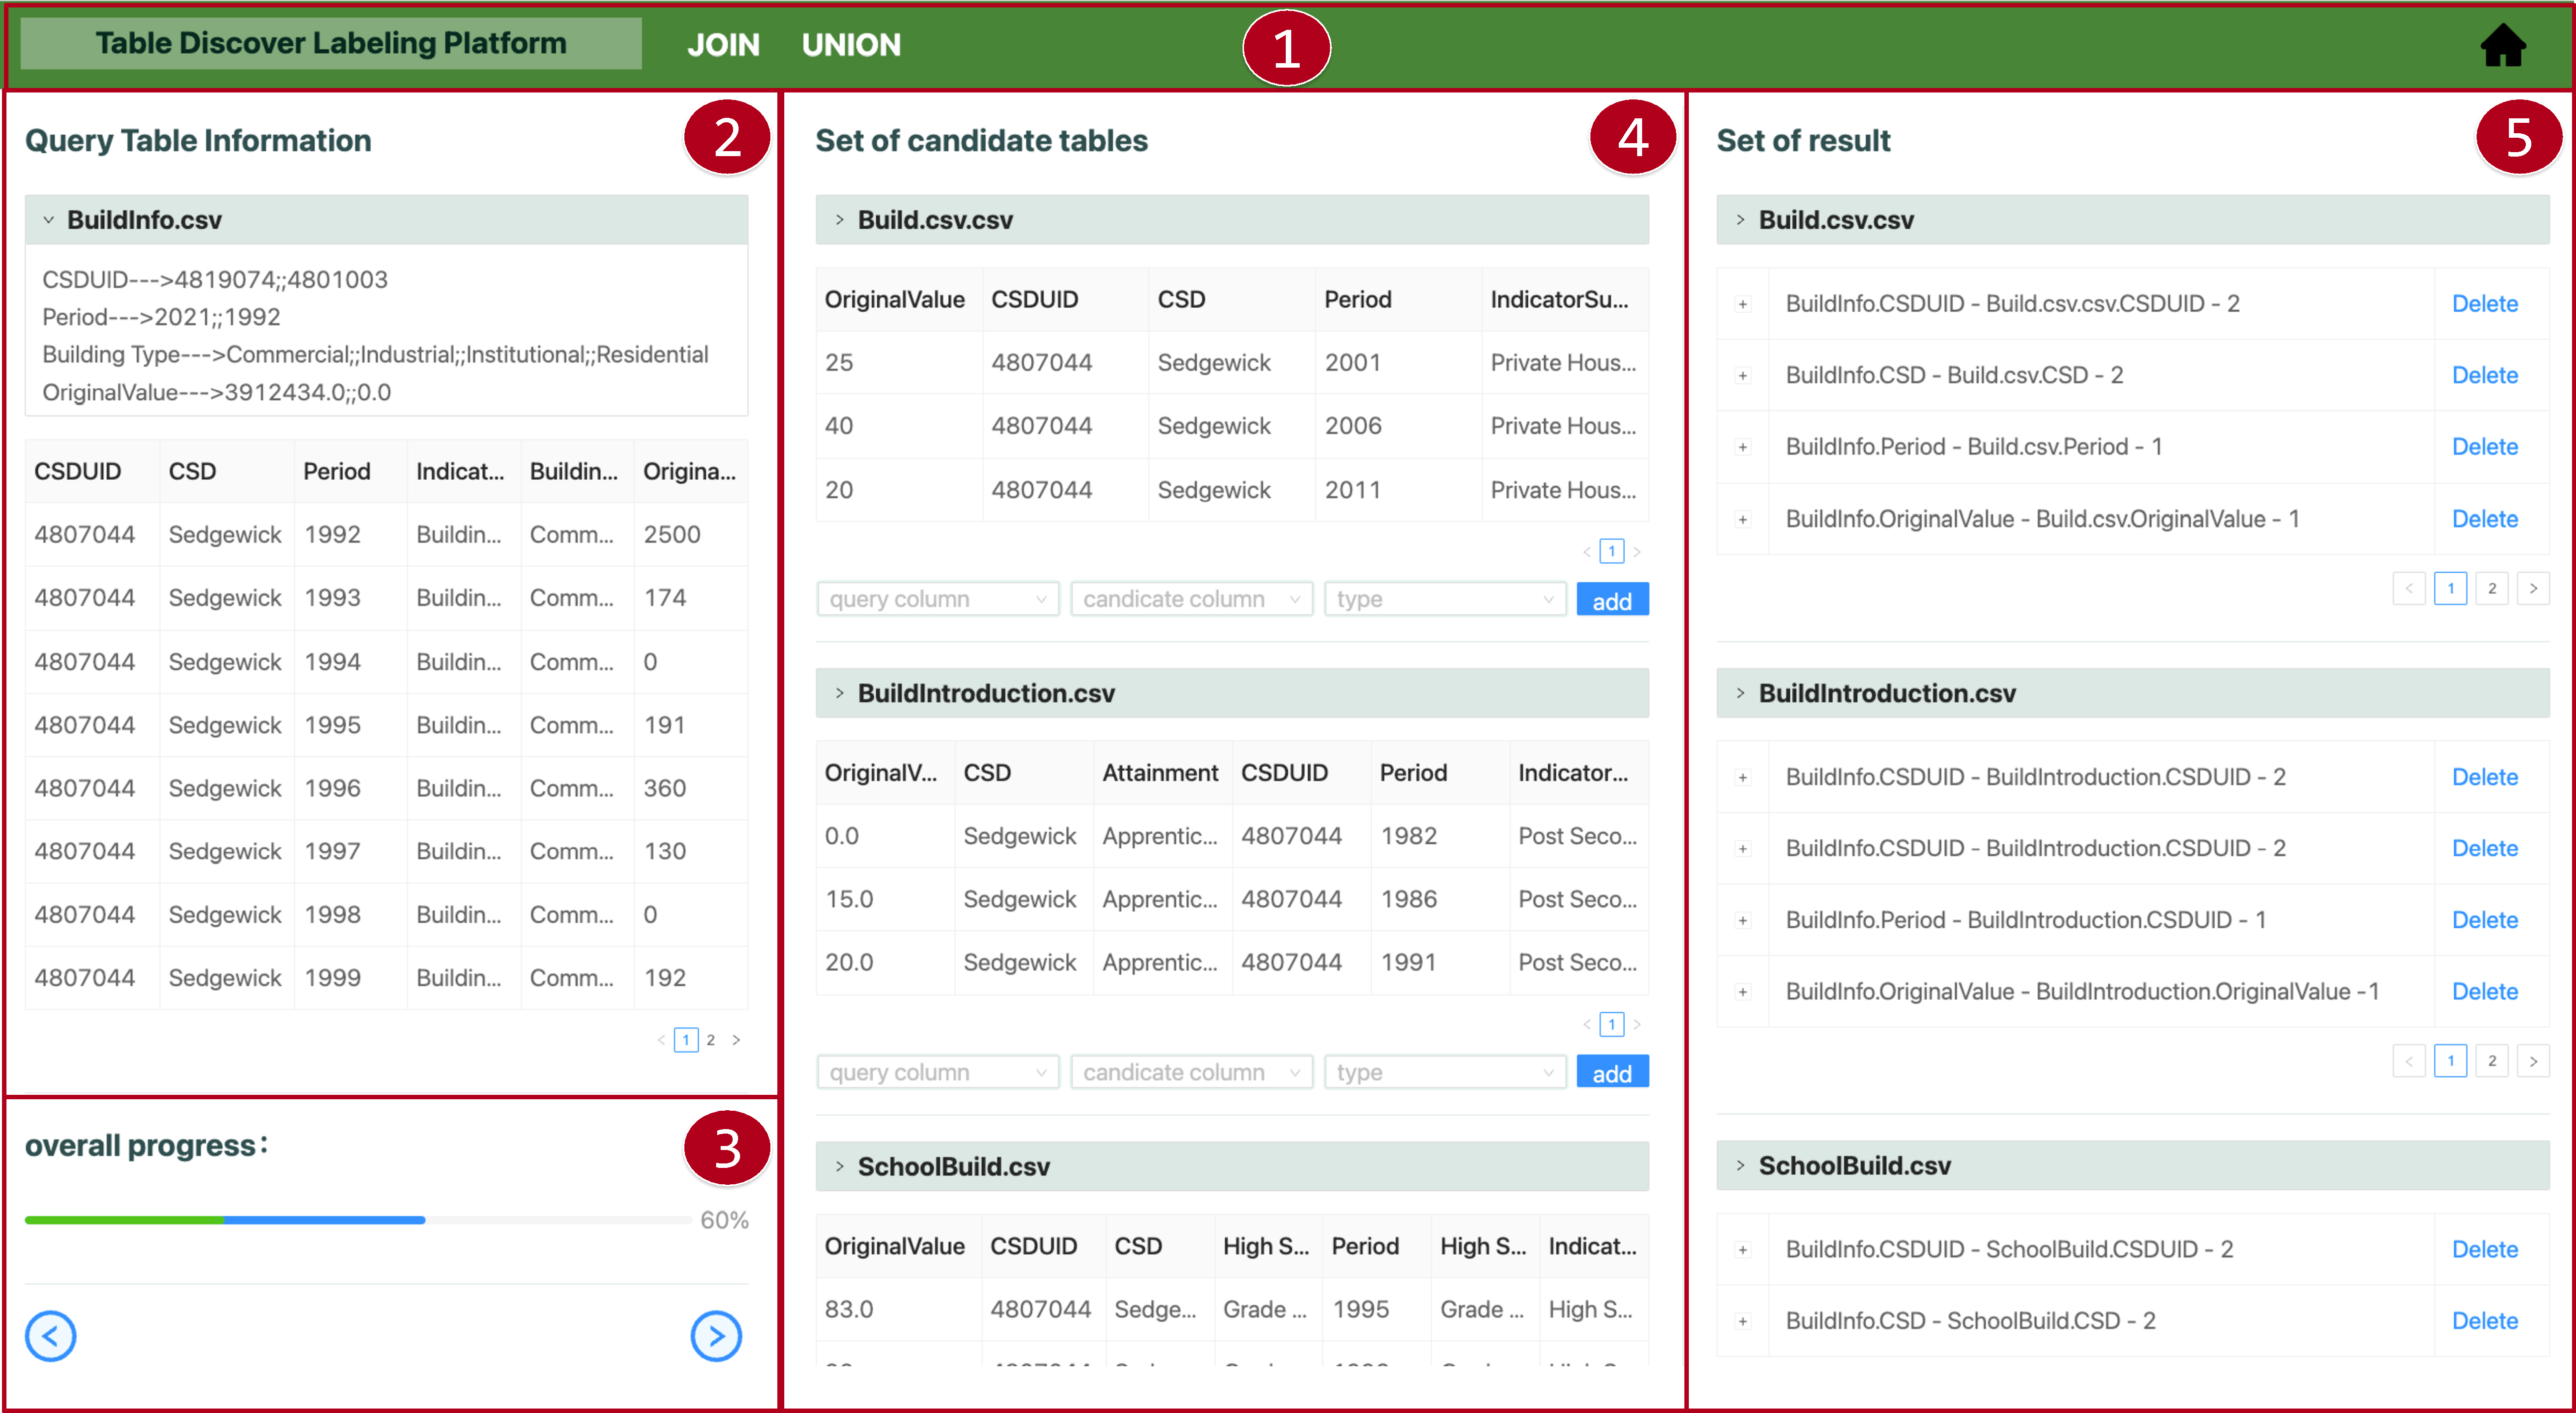
\includegraphics[width=1.0\linewidth]{fig/interface.pdf}
	\caption{Labeling Interface.}
	\label{fig:interface}
\end{figure*}

\noindent \textbf{Labeling Statistics.} 
We have count some statistical information during manual labeling, as show in Table ~\ref{Table:humanLabeling}. For OpenData Large, this dataset has a total of  \cc{XX} query tables to be labeled, with an average of 20 candidate tables matching each query table. Therefore, we have 10 experts and spent a total of approximately \cc{XX} hours completing the labeling work. Similarly, for WebTable Large, we also have 10 experts and spent a total of approximately \cc{XX} hours for labeling. This is because this dataset has \cc{XX} query tables in all that need to be labeled, and each table has an average of 20 corresponding candidate tables.

\begin{table}[t]
	\centering
	\caption{Statistics of Human Labeling.}
	\begin{tabular}{|c|c|c|c|c|c|}
		\hline
		\centering
		Data Lake  & \#-Query Tables & $\#$-People & Time.   \\
		\hline  
		OpenData Small& 914  & 10 & 10h   \\
		\hline
		OpenData Large& 1,448  & 10  &  17.5h   \\
		\hline
		WebTable Small& 1,745   & 10 &  20h  \\
		\hline
		WebTable Large& 2,245  & 10 &  30h  \\
		\hline
	\end{tabular}
	\label{Table:humanLabeling}
	
\end{table}